\documentclass[11pt, a4paper]{article}
\usepackage[utf8]{inputenc}
\usepackage[T1]{fontenc}
\usepackage[polish]{babel}
\usepackage{graphicx}
\usepackage{hyperref}
\usepackage{geometry}
\usepackage{longtable}
\usepackage{array}
\usepackage{enumitem}
\usepackage{float}
\usepackage{placeins} % \FloatBarrier
\usepackage{xcolor}
\usepackage{listings}
\lstset{
    literate=
    {ą}{{\k{a}}}1
    {ć}{{\'c}}1
    {ę}{{\k{e}}}1
    {ł}{{\l{}}}1
    {ń}{{\'n}}1
    {ó}{{\'o}}1
    {ś}{{\'s}}1
    {ź}{{\'z}}1
    {ż}{{\.z}}1
    {Ą}{{\k{A}}}1
    {Ć}{{\'C}}1
    {Ę}{{\k{E}}}1
    {Ł}{{\L{}}}1
    {Ń}{{\'N}}1
    {Ó}{{\'O}}1
    {Ś}{{\'S}}1
    {Ź}{{\'Z}}1
    {Ż}{{\.Z}}1
}
% --- Listing styles used in API examples ---
\lstdefinestyle{http}{
  basicstyle=\ttfamily\small,
  breaklines=true,
  frame=single,
  columns=fullflexible
}
\lstdefinestyle{json}{
  basicstyle=\ttfamily\small,
  breaklines=true,
  frame=single,
  columns=fullflexible
}


\geometry{margin=2.5cm}

\title{\textbf{Finalna wersja specyfikacji}\\ \large FlatShare}
\author{Grupa projektowa: \\ Jakub Rak, Bartosz Radomski, Sofiia Kuzmenko, Piotr Wójcik}
\date{}

\begin{document}

\maketitle

\begin{figure}[h!]
\centering
\includegraphics[width=\textwidth]{flatshare_final.png}
\end{figure}

\newpage
\tableofcontents
\newpage

\section{Wstęp}
Dokument zawiera specyfikację wymagań funkcjonalnych oraz projekt architektury systemu. Celem systemu jest połączenie właścicieli mieszkań z potencjalnymi lokatorami poprzez mechanizmy dopasowania preferencji oraz bezpośrednią komunikację. System jest podzielony na niezależne moduły, które komunikują się poprzez warstwę serwisową.


\subsection{Cel i ogólna koncepcja systemu}
FlatShare odpowiada na typowy problem rynku najmu pokoi: duża liczba ogłoszeń, brak ustandaryzowanej informacji o preferencjach domowników oraz konieczność wielokrotnej, powtarzalnej komunikacji przed podjęciem decyzji o wynajmie. System ma zmniejszyć „tarcie” po obu stronach procesu:
\begin{itemize}
    \item \textbf{Lokator} szybciej znajduje ogłoszenia pasujące do jego potrzeb (filtry + dopasowywanie) oraz ma bezpośredni kanał kontaktu z właścicielem.
    \item \textbf{Właściciel} publikuje ogłoszenia w spójnej formie, kontroluje dostępność i może akceptować rezerwacje lub włączyć tryb \textit{Instant Book}.
    \item \textbf{Administrator} utrzymuje jakość platformy poprzez obsługę zgłoszeń naruszeń i blokowanie kont łamiących regulamin.
\end{itemize}

\subsection{Zakres funkcjonalny i granice systemu}
Zakres systemu obejmuje trzy główne obszary: (1) ogłoszenia i wyszukiwanie, (2) komunikację i profilowanie użytkowników, (3) rezerwacje oraz płatności. W ramach projektu zakłada się, że:
\begin{itemize}
    \item System obsługuje \textbf{wynajem pokoju} w ramach mieszkania (model \texttt{Apartment/Room}).
    \item Dane o płatnościach są przetwarzane \textbf{pośrednio} --- FlatShare inicjuje płatność i utrzymuje jej status, natomiast właściwe obciążenie realizuje zewnętrzna bramka płatnicza.
    \item Zdjęcia ogłoszeń są przechowywane w zewnętrznym magazynie plików (np. obiektowe \textit{file storage}), a system przechowuje referencje/URL-e.
\end{itemize}
Poza zakresem (w tej iteracji) pozostają m.in.: generowanie umów najmu, rozbudowane rozliczenia cykliczne (czynsz co miesiąc), zaawansowany KYC użytkowników oraz wielowalutowe rozliczenia z przewalutowaniem.

\subsection{Wysokopoziomowa struktura systemu}
System jest projektowany jako aplikacja z rozdzieleniem na warstwy: \textbf{kontrolery REST} (wejście HTTP), \textbf{serwisy aplikacyjne} (logika przypadków użycia) oraz \textbf{repozytoria} (trwałość danych). Dodatkowo wydzielono porty integracyjne (np. bramka płatności, powiadomienia) w celu utrzymania niskiego sprzężenia pomiędzy logiką domenową a infrastrukturą. Taki podział jest widoczny na diagramach klas i modułów w dalszej części dokumentu.

\subsection{Spójność pomiędzy wymaganiami, domeną i API}
W dalszych rozdziałach wymagania (historie użytkownika) są mapowane na przypadki użycia, a następnie na obiekty domenowe (np. \texttt{Listing}, \texttt{Booking}, \texttt{Payment}) oraz endpointy API. Dzięki temu jedna funkcjonalność ma jedno „źródło prawdy” w modelu domenowym, a diagramy sekwencji i przykładowe komunikaty API odzwierciedlają te same reguły biznesowe (np. rezerwacja przechodzi do \texttt{CONFIRMED} dopiero po sukcesie płatności).

\section{Historie Użytkownika (User Stories)}
Poniżej przedstawiono wymagania biznesowe zagregowane według aktorów systemu.

\subsection{Aktor: Użytkownik (Wspólne)}
\begin{itemize}
    \item \textbf{US-Sys1:} Jako Użytkownik, chcę bezpiecznie logować się do systemu, aby uzyskać dostęp do swojego konta.
    \item \textbf{US-Sys2:} Jako Użytkownik, chcę mieć możliwość resetu hasła, aby odzyskać dostęp do konta w przypadku jego zapomnienia.
\end{itemize}

\subsection{Aktor: Lokator}
\begin{itemize}
    \item \textbf{US-L1:} Jako Lokator, chcę przeglądać i filtrować ogłoszenia (wg ceny, lokalizacji), aby szybko znaleźć pokój spełniający moje kryteria.
    \item \textbf{US-L2:} Jako Lokator, chcę zdefiniować swoje preferencje (np. zwierzęta, palenie), aby system mógł podpowiadać mi najlepiej dopasowane oferty.
    \item \textbf{US-L4:} Jako Lokator, chcę wysłać prośbę o rezerwację pokoju, aby sfinalizować proces wynajmu.
    \item \textbf{US-L5:} Jako Lokator, chcę opłacić rezerwację przez zewnętrzny system płatności, aby potwierdzić wynajem.
\end{itemize}

\subsection{Aktor: Właściciel Mieszkania}
\begin{itemize}
    \item \textbf{US-W1:} Jako Właściciel, chcę wystawić ogłoszenie ze zdjęciami i opisem, aby dotrzeć do potencjalnych najemców.
    \item \textbf{US-W2:} Jako Właściciel, chcę określić preferowany profil lokatora (np. student, osoba pracująca), aby uniknąć nieporozumień.
    \item \textbf{US-W3:} Jako Właściciel, chcę zarządzać dostępnością ogłoszenia (publikować/ukrywać/archiwizować), gdy mieszkanie zostanie wynajęte.
    \item \textbf{US-W4:} Jako Właściciel, chcę zaakceptować lub odrzucić rezerwację, aby kontrolować kto wynajmuje pokój.
    \item \textbf{US-W5:} Jako Właściciel, chcę włączyć opcję \textit{Instant Book}, aby automatyzować rezerwacje bez ręcznej akceptacji.
\end{itemize}

\subsection{Aktor: Administrator}
\begin{itemize}
    \item \textbf{US-A1:} Jako Admin, chcę mieć możliwość blokowania użytkowników łamiących regulamin, aby utrzymać porządek w serwisie.
    \item \textbf{US-A2:} Jako Admin, chcę przeglądać zgłoszone naruszenia w panelu administracyjnym, aby szybko reagować na nadużycia.
\end{itemize}


\subsection{Kryteria akceptacji dla kluczowych historii użytkownika}
Poniższe kryteria akceptacji stanowią „rewersy” historii użytkownika i są wykorzystywane jako
podstawa do weryfikacji implementacji. W kryteriach celowo pojawiają się terminy z domeny
(\texttt{Listing}, \texttt{Booking}, \texttt{Payment}, \texttt{MessageThread}), aby zachować spójność
z dalszym opisem modeli, stanów oraz komunikacji API.

\subsubsection{US-Sys1: Bezpieczne logowanie (JWT)}
\begin{itemize}
    \item \textbf{AC1:} Dla aktywnego użytkownika z poprawnymi danymi uwierzytelniającymi system zwraca \texttt{200 OK} oraz token JWT zawierający identyfikator użytkownika i role.
    \item \textbf{AC2:} Dla błędnego loginu lub hasła system zwraca \texttt{401 Unauthorized} bez ujawniania informacji o tym, czy konto istnieje.
    \item \textbf{AC3:} Token jest wymagany dla endpointów chronionych, a brak tokenu skutkuje \texttt{401 Unauthorized}.
\end{itemize}

\subsubsection{US-W1: Wystawienie ogłoszenia}
\begin{itemize}
    \item \textbf{AC1:} Właściciel z rolą \texttt{LANDLORD} może utworzyć ogłoszenie z wymaganymi danymi (tytuł, opis, cena, lokalizacja, dostępność), a system przypisuje je do jego konta.
    \item \textbf{AC2:} System odrzuca niepoprawne dane (np. cena $\leq 0$) odpowiedzią \texttt{400 Bad Request} oraz zwraca listę błędów pól.
    \item \textbf{AC3:} Ponowienie tego samego żądania z identycznym \texttt{Idempotency-Key} nie powoduje utworzenia duplikatu ogłoszenia.
\end{itemize}

\subsubsection{US-L2: Zdefiniowanie preferencji i dopasowywanie}
\begin{itemize}
    \item \textbf{AC1:} Lokator może zapisać zestaw preferencji (np. palenie, zwierzęta, budżet), a system przechowuje je w kontekście roli \texttt{TenantRole}.
    \item \textbf{AC2:} Endpoint dopasowań zwraca ogłoszenia posortowane malejąco po \textit{match score}.
    \item \textbf{AC3:} Jeśli preferencje nie są ustawione, system zwraca pustą listę (lub zgodnie z polityką --- \texttt{404 Not Found}).
\end{itemize}

\subsubsection{US-L4/US-W4: Rezerwacja i akceptacja/odrzucenie}
\begin{itemize}
    \item \textbf{AC1:} Lokator może złożyć prośbę o rezerwację tylko dla ogłoszenia w stanie \texttt{ACTIVE} i dostępnego terminu.
    \item \textbf{AC2:} Właściciel może zaakceptować lub odrzucić rezerwację; decyzja zmienia stan \texttt{Booking} odpowiednio na \texttt{PENDING\_PAYMENT} lub \texttt{REJECTED}.
    \item \textbf{AC3:} Wariant \textit{Instant Book} pomija etap akceptacji i przechodzi bezpośrednio do \texttt{PENDING\_PAYMENT}.
\end{itemize}

\subsubsection{US-L5: Płatność za rezerwację}
\begin{itemize}
    \item \textbf{AC1:} System inicjuje płatność w bramce zewnętrznej i zapisuje obiekt \texttt{Payment} w stanie \texttt{Initiated/Redirected}.
    \item \textbf{AC2:} Po potwierdzeniu płatności status \texttt{Payment} zmienia się na \texttt{Succeeded}, a \texttt{Booking} na \texttt{CONFIRMED}.
    \item \textbf{AC3:} Nieudana płatność skutkuje \texttt{Failed} oraz mapowaniem na \texttt{PAYMENT\_FAILED} po stronie \texttt{Booking}; użytkownik może ponowić próbę.
\end{itemize}

\subsubsection{US-A1/US-A2: Moderacja i blokada użytkownika}
\begin{itemize}
    \item \textbf{AC1:} Administrator widzi listę zgłoszeń naruszeń wraz ze statusem sprawy (\texttt{Open/UnderReview/...}).
    \item \textbf{AC2:} Zablokowanie użytkownika ustawia \texttt{User.status = BLOCKED} oraz ukrywa jego aktywne ogłoszenia.
    \item \textbf{AC3:} Zablokowany użytkownik nie może tworzyć nowych ogłoszeń ani wysyłać wiadomości; próba skutkuje \texttt{403 Forbidden}.
\end{itemize}


\section{Diagramy Przypadków Użycia (Use Cases)}
Funkcjonalności zostały podzielone na logiczne moduły, co ułatwia analizę systemu. Diagramy przypadków użycia stanowią ilustrację do wstępów poszczególnych grup funkcjonalności.

\subsection{Moduł Ogłoszeń}
\begin{figure}[H]
    \centering
    \includegraphics[width=0.4\linewidth]{diagram_listings.png}
    \caption{Diagram przypadków użycia - Moduł Ogłoszeń}
\end{figure}


\noindent\textbf{Opis modułu.} Moduł Ogłoszeń koncentruje się na zarządzaniu zasobem \texttt{Listing}
oraz jego prezentacji po stronie Lokatora. Jak pokazuje rysunek, Lokator może przeglądać ogłoszenia,
korzystać z filtrów oraz przechodzić do szczegółów wybranego ogłoszenia. Równolegle system udostępnia
widok rekomendacji (\textit{matching}), który wykorzystuje preferencje Lokatora do wyliczenia dopasowania.

\noindent\textbf{Główne funkcje po stronie Lokatora:}
\begin{itemize}
    \item \textit{Przeglądaj ogłoszenia} --- podstawowa lista ofert, stanowiąca punkt startowy dla dalszych akcji.
    \item \textit{Szukaj / filtruj ogłoszenia} --- zawężanie wyników m.in. po cenie i lokalizacji (realizacja US-L1).
    \item \textit{Wyświetl szczegóły ogłoszenia} --- wejście w kontekst konkretnego \texttt{Listing}, niezbędne m.in. do wiadomości i rezerwacji.
    \item \textit{Wyświetl rekomendacje / matching} --- wariant listy ofert posortowanej po \textit{match score} (powiązanie z US-L2).
\end{itemize}

\noindent\textbf{Główne funkcje po stronie Właściciela:}
\begin{itemize}
    \item \textit{Dodaj ogłoszenie} oraz \textit{Edytuj ogłoszenie} --- przygotowanie kompletnej oferty do publikacji (US-W1).
    \item \textit{Ukryj lub archiwizuj ogłoszenie} --- kontrola dostępności i zakończenie cyklu życia ogłoszenia (US-W3), spójne ze stanami \texttt{Hidden/Archived} opisanymi później.
\end{itemize}

\noindent W kolejnych rozdziałach diagramy stanów i aktywności doprecyzowują, kiedy ogłoszenie jest widoczne
(\texttt{ACTIVE}) i jakie akcje są dozwolone w poszczególnych stanach.



\subsection{Moduł Użytkownika}
\begin{figure}[H]
    \centering
    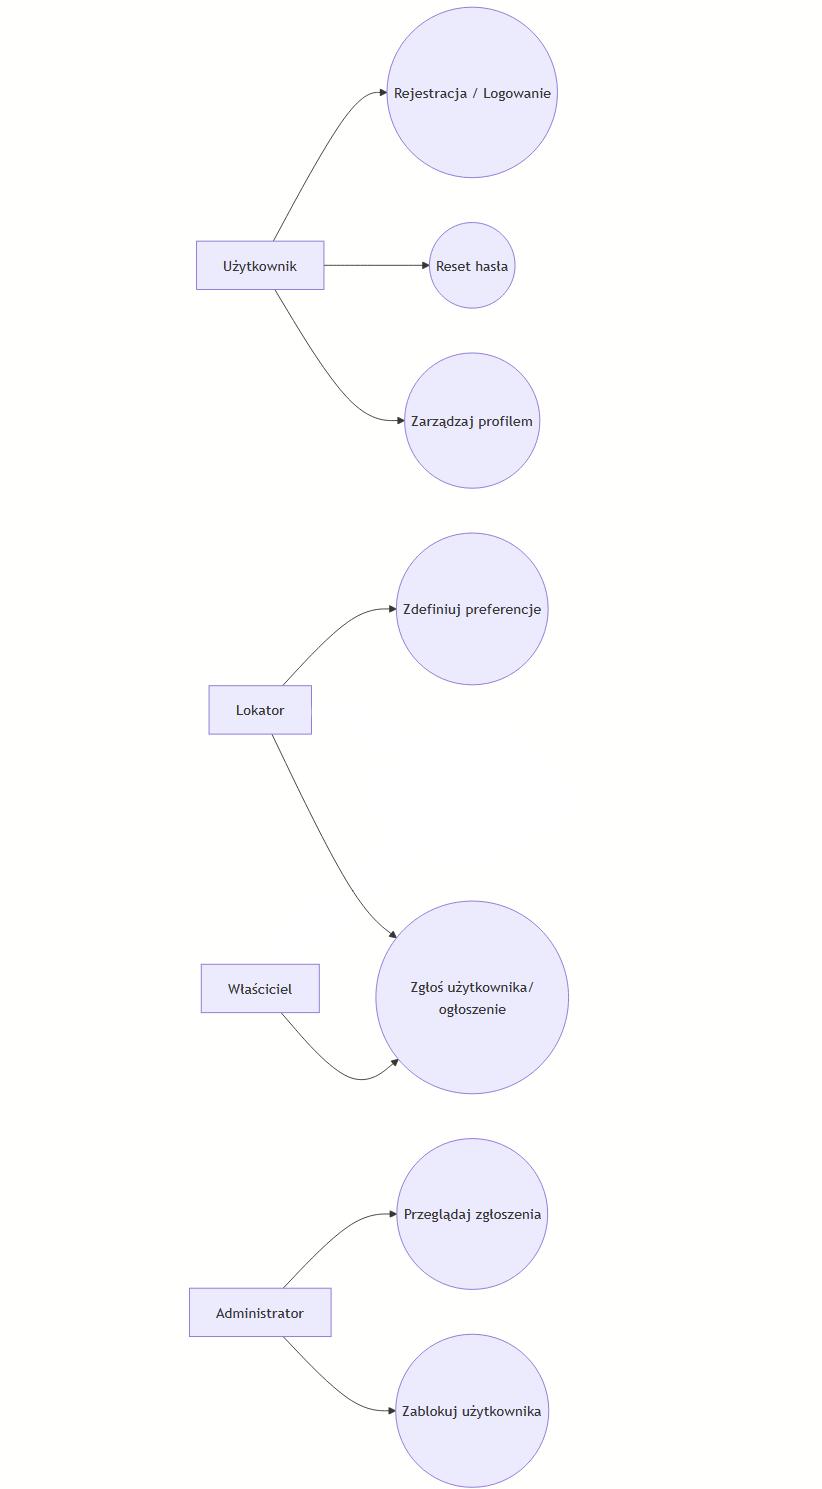
\includegraphics[width=0.65\linewidth]{diagram_accounts_messaging.png}
    \caption{Diagram przypadków użycia - Moduł Użytkownika i Komunikacji}
\end{figure}


\noindent\textbf{Opis modułu.} Moduł Użytkownika łączy funkcje związane z kontem (\texttt{User}),
rolami oraz wymianą wiadomości pomiędzy Lokatorem i Właścicielem. Z perspektywy bezpieczeństwa
to właśnie w tym obszarze powstaje token JWT wykorzystywany później przez pozostałe moduły.

\noindent\textbf{Zarządzanie kontem:} rejestracja/logowanie, reset hasła oraz zarządzanie profilem stanowią funkcje wspólne,
niezależne od roli użytkownika. Profil obejmuje dane kontaktowe i ustawienia, natomiast \texttt{User.status} determinuje,
czy użytkownik może korzystać z systemu (np. \texttt{BLOCKED} po moderacji).

\noindent\textbf{Preferencje i dopasowanie:} Lokator może zdefiniować preferencje, które są wykorzystywane przez moduł dopasowań
do wyliczenia rekomendacji. Ważne jest rozdzielenie danych „kontowych” od danych roli --- preferencje są przechowywane
w \texttt{TenantRole}, co jest spójne z modelem domenowym.

\noindent\textbf{Zgłoszenia:} 
Zarówno Lokator, jak i Właściciel mogą zgłosić użytkownika lub ogłoszenie, co inicjuje
proces moderacyjny obsługiwany przez Administratora.


\subsection{Moduł Wynajmu i Płatności}
\begin{figure}[H]
    \centering
    \includegraphics[width=0.6\linewidth]{diagram_booking_payments.png}
    \caption{Diagram przypadków użycia - Moduł Wynajmu/Rezerwacji i Płatności (realizacja US-L4, US-L5, US-W4, US-W5)}
\end{figure}


\noindent\textbf{Opis modułu.} Moduł Wynajmu i Płatności obejmuje pełny przepływ rezerwacji pokoju: od złożenia prośby,
przez decyzję Właściciela, aż po opłacenie i potwierdzenie. W module występują również integracje zewnętrzne:
\textbf{System Płatności} (realizacja obciążenia) oraz \textbf{Serwis Powiadomień} (informowanie stron o zdarzeniach).

\noindent\textbf{Rezerwacja jako obiekt biznesowy.} Kluczowym obiektem jest \texttt{Booking} (w API opisywany jako „wynajem”),
który przechowuje status procesu. Wariant standardowy wymaga akceptacji Właściciela (\texttt{PENDING\_APPROVAL}),
natomiast \textit{Instant Book} umożliwia automatyczne przejście do płatności (\texttt{PENDING\_PAYMENT}).

\noindent\textbf{Płatność i powiadomienia.} Płatność jest śledzona w osobnym obiekcie \texttt{Payment} i wpływa na stan rezerwacji.
W praktyce moduł wysyła powiadomienia po kluczowych zdarzeniach: utworzenie rezerwacji, akceptacja/odrzucenie,
sukces/porażka płatności oraz anulowanie. Dzięki temu obie strony mają spójny obraz postępu procesu.

\subsection{Moduł moderacji}
\begin{figure}[H]
    \centering
    \includegraphics[width=0.5\linewidth]{obraz.png}
\caption{Moderacja — przypadki użycia}
\end{figure}


\noindent\textbf{Opis modułu.} Moduł moderacji odpowiada za utrzymanie jakości platformy oraz reagowanie na nadużycia.
Proces zaczyna się od zgłoszenia naruszenia (obiekt \texttt{ViolationReport}), a następnie przechodzi przez analizę Administratora
i kończy się decyzją: zamknięcie bez akcji lub podjęcie działań (np. blokada konta).

\noindent\textbf{Konsekwencje blokady.} Zablokowanie użytkownika jest decyzją systemową o skutkach wielomodułowych:
\begin{itemize}
    \item \texttt{User.status} przechodzi do \texttt{BLOCKED}, co ogranicza dostęp do endpointów chronionych dla danego użytkownika,
    \item aktywne ogłoszenia są ukrywane (\texttt{Listing} $\rightarrow$ \texttt{HiddenByModeration} lub równoważny stan „ukryty”),
    \item system wysyła powiadomienie o blokadzie, aby zapewnić transparentność procesu.
\end{itemize}
Dalsze diagramy stanów i aktywności pokazują, jak te konsekwencje propagują się do cyklu życia konta i ogłoszeń.


\section{Szczegółowa specyfikacja (Deep Dive)}
Szczegółowy opis kluczowych przypadków użycia wg szablonu Cockburna (główne scenariusze oraz kluczowe alternatywy).

\subsection{Przypadek: Wystawienie ogłoszenia}
\begin{longtable}{|p{4cm}|p{10cm}|}
\hline
\textbf{Nazwa przypadku} & \textbf{Wystawienie ogłoszenia (Create Listing)} \\ \hline
\textbf{Aktor główny} & Właściciel Mieszkania \\ \hline
\textbf{Aktorzy pomocniczy} & System Przechowywania Plików (File Storage), (opcjonalnie) System Płatności \\ \hline
\textbf{Warunki wstępne} & Użytkownik zalogowany, posiada rolę Właściciela. \\ \hline
\textbf{Główny scenariusz} &
1. Właściciel wybiera opcję ``Dodaj ogłoszenie''. \newline
2. System prosi o dane (tytuł, opis, cena, lokalizacja) oraz zdjęcia. \newline
3. Właściciel wprowadza dane i dodaje zdjęcia. \newline
4. System waliduje dane (np. cena > 0, wymagane pola). \newline
5. System zapisuje ogłoszenie (status: \textit{DRAFT} lub \textit{UNDER\_REVIEW} zgodnie z polityką). \newline
6. (Jeśli dotyczy) System publikuje ogłoszenie (status: \textit{ACTIVE}).
\\ \hline
\textbf{Scenariusze alternatywne} &
\textbf{4a. Błąd walidacji:} System wyświetla błędy i prosi o poprawę. \newline
\textbf{5a. Limit darmowych publikacji:} Jeśli użytkownik przekroczył limit darmowych ogłoszeń, system przechodzi do płatności i dopiero po sukcesie umożliwia publikację.
\\ \hline
\end{longtable}
\subsection{Przypadek: Rezerwacja pokoju (z płatnością)}
\begin{longtable}{|p{4cm}|p{10cm}|}
\hline
\textbf{Nazwa przypadku} & \textbf{Rezerwacja pokoju (Book a Room)} \\ \hline
\textbf{Aktor główny} & Lokator \\ \hline
\textbf{Aktorzy pomocniczy} & Właściciel, System Płatności (zewnętrzny), Serwis Powiadomień \\ \hline
\textbf{Warunki wstępne} & Lokator zalogowany, ogłoszenie ma status ACTIVE, pokój dostępny dla wybranego okresu. \\ \hline
\textbf{Główny scenariusz} &
1. Lokator na stronie ogłoszenia klika ``Rezerwuj''. \newline
2. System pokazuje podsumowanie kosztów, regulamin i prosi o potwierdzenie. \newline
3. Lokator potwierdza chęć rezerwacji. \newline
4. System tworzy rezerwację ze statusem \texttt{PENDING\_APPROVAL} i wysyła powiadomienie do Właściciela. \newline
5. Właściciel akceptuje rezerwację. \textcolor{red}{System zmienia status na \texttt{PENDING\_PAYMENT}, tymczasowo blokuje termin (uruchamia licznik czasu) i generuje link do płatności.} \newline
6. System przekierowuje Lokatora do Systemu Płatności. \newline
7. System Płatności potwierdza płatność. System zmienia status rezerwacji na \texttt{CONFIRMED} \textcolor{red}{(blokada terminu staje się stała).} \newline
8. Serwis Powiadomień wysyła potwierdzenia do Lokatora i Właściciela.
\\ \hline
\textbf{Scenariusze alternatywne} &
\textbf{4a. Instant Book:} Jeśli Właściciel włączył Instant Book, system pomija akceptację: rezerwacja powstaje od razu jako \texttt{PENDING\_PAYMENT}, \textcolor{red}{blokuje termin} i przechodzi do kroku 6. \newline
\textbf{5b. Brak reakcji/Timeout płatności:} Właściciel nie odpowiada lub \textcolor{red}{Lokator nie opłaci rezerwacji w wyznaczonym czasie (np. 15 min)}. System ustawia status \texttt{EXPIRED}, \textcolor{red}{zwalnia blokadę terminu} i powiadamia Lokatora. \newline
\textbf{7a. Błąd płatności:} Płatność nieudana. System ustawia status \texttt{PAYMENT\_FAILED} i umożliwia ponowienie lub anulowanie.
\\ \hline
\end{longtable}

\subsection{Przypadek: Blokada użytkownika (Moderacja)}
\begin{longtable}{|p{4cm}|p{10cm}|}
\hline
\textbf{Nazwa przypadku} & \textbf{Blokada użytkownika (Ban User)} \\ \hline
\textbf{Aktor główny} & Administrator \\ \hline
\textbf{Warunki wstępne} & Admin zalogowany do panelu administracyjnego. \\ \hline
\textbf{Główny scenariusz} &
1. Admin przegląda listę zgłoszeń naruszeń. \newline
2. Admin analizuje historię zgłoszonego użytkownika. \newline
3. Admin wybiera opcję ``Zablokuj konto'' i podaje powód. \newline
4. System zmienia status użytkownika na \textit{BLOCKED}. \newline
5. Wszystkie aktywne ogłoszenia użytkownika są ukrywane. \newline
6. \textcolor{red}{System wyszukuje aktywne rezerwacje (CONFIRMED) u zablokowanego właściciela, zmienia ich status na CANCELLED/REFUNDED i zleca zwrot środków.} \newline
7. Serwis Powiadomień wysyła wiadomość email z informacją o blokadzie \textcolor{red}{oraz o anulowaniu rezerwacji}.
\\ \hline
\textbf{Scenariusze alternatywne} &
\textbf{3a. Odrzucenie zgłoszenia:} Admin uznaje zgłoszenie za bezzasadne i zamyka sprawę bez blokady.
\\ \hline
\end{longtable}
\newpage
\section{Diagramy Klas i Architektura (Class Diagrams)}
Poniższe diagramy prezentują strukturę klas zaprojektowaną w celu realizacji funkcjonalności zdefiniowanych w diagramach przypadków użycia.
Projekt rozdziela modele danych (encje domenowe) od logiki (serwisy), zgodnie z zasadami SOLID.

\subsection{Model domenowy (encje i powiązania)}
\begin{figure}[H]
    \centering
    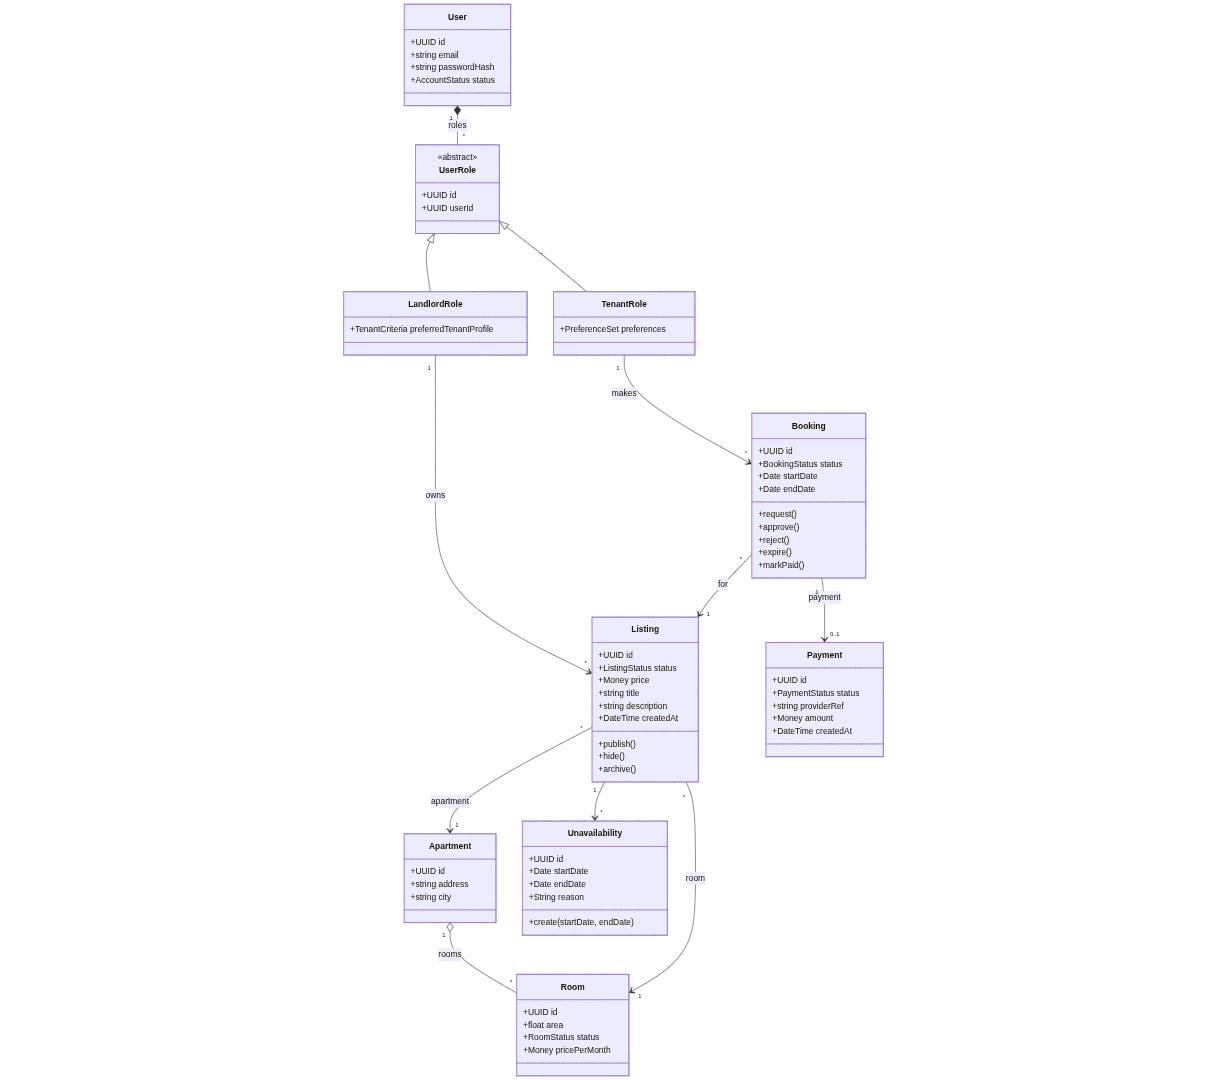
\includegraphics[width=0.9\linewidth]{class_domain_core.png}
    \caption{Diagram klas - model domenowy (User + Role, Listing, Apartment/Room, Booking, Payment)}
\end{figure}
\paragraph{Uwaga projektowa (spójność domeny).}
Rezerwacja (\texttt{Booking}) jest zawsze tworzona przez Lokatora (rola \texttt{TenantRole})
i dotyczy konkretnego ogłoszenia (\texttt{Listing}). Z tego powodu w modelu domenowym
\texttt{Booking} posiada powiązania do \texttt{TenantRole} oraz \texttt{Listing}.


\subsection{Warstwa serwisów i repozytoriów (DIP/OCP)}
\begin{figure}[H]
    \centering
    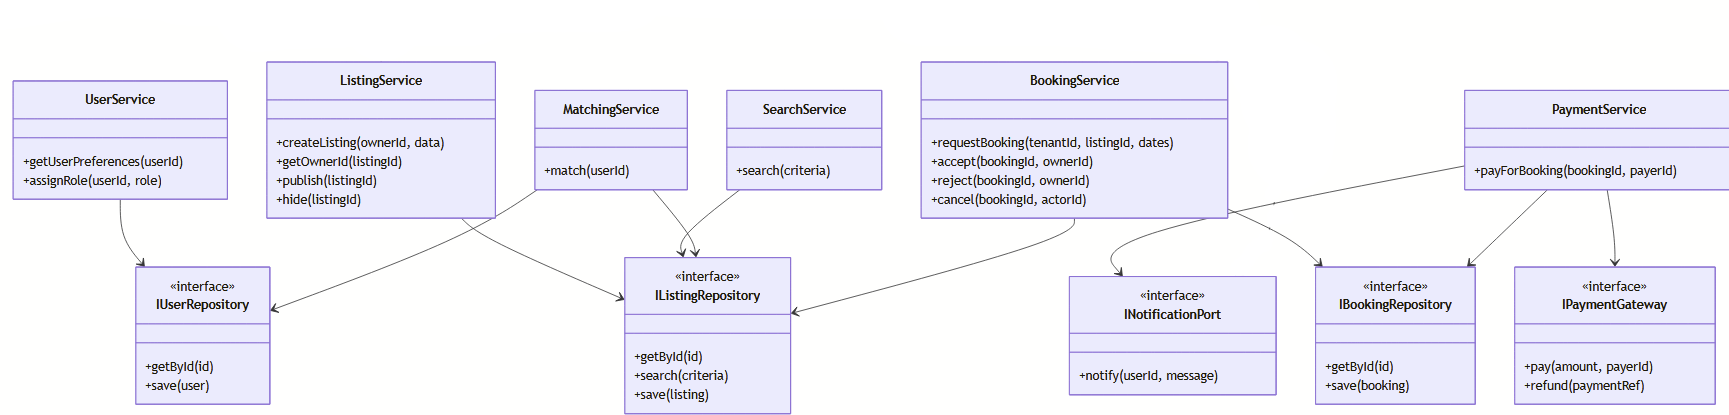
\includegraphics[width=0.9\linewidth]{class_services_repos.png}
    \caption{Diagram klas - serwisy, repozytoria i porty integracyjne (płatności, powiadomienia)}
\end{figure}

\subsection{Moduły i komunikacja}
\begin{figure}[H]
    \centering
    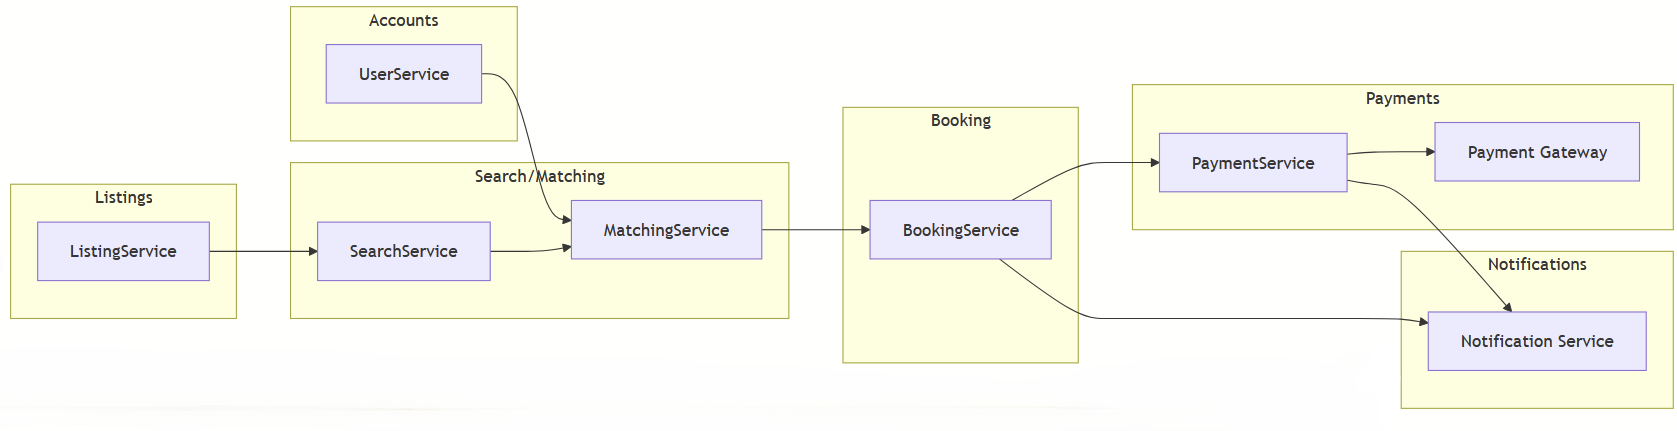
\includegraphics[width=0.95\linewidth]{modules_communication.png}
    \caption{Podział na moduły i kanały komunikacji (inter-module communication)}
\end{figure}

\noindent\textbf{Interpretacja diagramu modułów.} Moduły na rysunku należy rozumieć jako \textbf{logiczne komponenty}
w obrębie jednej aplikacji serwerowej (nie jako osobne mikroserwisy). Dzięki temu komunikacja pomiędzy modułami
realizowana jest przez jawne interfejsy serwisów i porty integracyjne, co ogranicza sprzężenie i ułatwia testowanie.

\noindent\textbf{Kanały komunikacji:}
\begin{itemize}
    \item \textbf{Wywołania synchroniczne (in-process)} pomiędzy modułami, np.
    \item \textbf{Integracje zewnętrzne} poprzez porty, np. \texttt{IPaymentGateway} (płatności) oraz \texttt{INotificationPort} (powiadomienia).
\end{itemize}

\noindent\textbf{Warstwy aplikacji a moduły.} Każdy moduł posiada analogiczną strukturę: kontrolery REST (wejście),
serwisy aplikacyjne (logika przypadków użycia) oraz repozytoria (dostęp do danych). Wspólny model domenowy jest
wykorzystywany w serwisach, natomiast „zewnętrzny świat” (HTTP, bazy danych, bramki) jest izolowany w warstwie infrastruktury.
Takie podejście jest spójne z przedstawioną dalej warstwą serwisów i repozytoriów (DIP/OCP).
\subsection{Kluczowe klasy i ich odpowiedzialność}
Zgodnie z wymaganiami projektowymi, system opiera się na obiektach domenowych oraz serwisach zarządzających logiką.

\begin{enumerate}
    \item \textbf{Użytkownicy i Role (Kompozycja):}
    \begin{itemize}
        \item Zamiast dziedziczenia ról od \texttt{User}, zastosowano kompozycję: \texttt{User} posiada przypisane obiekty ról (np. \texttt{TenantRole}, \texttt{LandlordRole}).
        \item \texttt{User} przechowuje dane uwierzytelniające oraz status konta.
        \item Role definiują uprawnienia i kontekst danych: preferencje należą do roli Lokatora, a zarządzanie mieszkaniami/ogłoszeniami do roli Właściciela.
    \end{itemize}

    \item \textbf{Ogłoszenia (Listing) oraz struktura lokalu:}
    \begin{itemize}
        \item \texttt{Listing} reprezentuje ogłoszenie powiązane z \texttt{Apartment} i \texttt{Room}.
        \item \textbf{Status ogłoszenia:} \texttt{Listing.status} (np. \textit{ACTIVE, HIDDEN, ARCHIVED}) pozwala zarządzać dostępnością i publikacją.
    \end{itemize}

    \item \textcolor{red}{\textbf{Zarządzanie dostępnością (Unavailability):}}
    \begin{itemize}
        \item \textcolor{red}{Wprowadzono encję \texttt{Unavailability} powiązaną relacją jeden-do-wielu z \texttt{Listing}.}
        \item \textcolor{red}{Pozwala ona Właścicielowi na wyłączenie konkretnych zakresów dat z wynajmu (np. remont, użytek własny) bez konieczności usuwania ogłoszenia czy tworzenia fikcyjnych rezerwacji.}
    \end{itemize}

    \item \textbf{Wynajem/Rezerwacja i Płatność:}
    \begin{itemize}
        \item \texttt{Booking} reprezentuje proces rezerwacji i przechowuje status (np. \textit{PENDING\_APPROVAL, PENDING\_PAYMENT, CONFIRMED}).
        \item \texttt{Payment} przechowuje wynik integracji z bramką płatności (referencja dostawcy, status).
    \end{itemize}
\end{enumerate}
\subsection{Wymiana informacji między modułami (Inter-module communication)}
System realizuje komunikację między niezależnymi modułami poprzez warstwę serwisową i porty integracyjne (interfejsy), aby moduły nie były bezpośrednio ze sobą sprzężone.

\begin{itemize}
    \item \textbf{Moduł Dopasowań $\leftarrow$ Moduł Użytkownika (Preferencje)}
    \newline
    Aby dopasować ogłoszenia do Lokatora, \texttt{MatchingService} potrzebuje preferencji Lokatora.
    \newline
    \textit{Wymagana interakcja:} \texttt{MatchingService} pobiera dane poprzez \texttt{UserService.getUserPreferences(userId)}.

    \item \textbf{Moduł Wynajmu $\rightarrow$ Moduł Płatności (integracja zewnętrzna)}
    \newline
    Aby potwierdzić rezerwację, moduł wynajmu inicjuje płatność w zewnętrznej bramce.
    \newline
    \textit{Wymagana interakcja:} \texttt{PaymentService.payForBooking(bookingId, payerId)} korzysta z portu \texttt{IPaymentGateway}.

    \item \textbf{Moduł Wynajmu/Płatności $\rightarrow$ Moduł Powiadomień}
    \newline
    Po kluczowych zdarzeniach (złożenie rezerwacji, akceptacja/odrzucenie, płatność) system powiadamia użytkowników.
    \newline
    \textit{Wymagana interakcja:} \texttt{BookingService} i \texttt{PaymentService} korzystają z portu \texttt{INotificationPort}.
\end{itemize}

% =========================
% Checkpoint 2 content
% =========================
\section{Diagramy stanów i aktywności}

\subsection{Cel i zakres}
Celem jest przedstawienie:
\begin{itemize}
  \item cyklu życia kluczowych obiektów biznesowych w formie diagramów stanów (wraz ze stanami szczególnymi oraz nietypowymi przejściami),
  \item kluczowych, powtarzalnych procesów biznesowych systemu w formie diagramów aktywności (z główną ścieżką i alternatywami).
\end{itemize}

W systemie FlatShare kluczowe procesy dotyczą: publikacji ogłoszeń, rezerwacji i płatności, komunikacji Lokatora z Właścicielem oraz moderacji (blokady użytkownika i obsługi zgłoszeń naruszeń).

% ---------------------------------------------------------
\subsection{Diagramy stanów kluczowych obiektów biznesowych}

\subsubsection{Obiekt: \texttt{User} (konto użytkownika)}
\begin{figure}[H]
  \centering
  \includegraphics[width=\linewidth]{state_user.png}
  \caption{Diagram stanów: \texttt{User}.}
  \label{fig:state-user}
\end{figure}

\textbf{Opis:} Diagram pokazuje cykl życia konta użytkownika. Standardowo konto przechodzi do stanu \texttt{Active} po rejestracji i/lub poprawnym uwierzytelnieniu. Uwzględniono stan szczególny \texttt{Blocked}, który wynika z decyzji administratora (moderacja) i uniemożliwia korzystanie z systemu.
\begin{itemize}
  \item \textbf{Ścieżka standardowa:} \texttt{Active} jako stan roboczy, w którym użytkownik korzysta z funkcji systemu.
  \item \textbf{Nietypowe przejścia:} reset hasła (\texttt{ResetRequested} $\rightarrow$ \texttt{Active}), blokada konta (\texttt{Active} $\rightarrow$ \texttt{Blocked}).
  \item \textbf{Stan końcowy:} \texttt{Deleted} (zamknięcie konta i zakończenie cyklu życia).
\end{itemize}

\FloatBarrier

\subsubsection{Obiekt: \texttt{Listing} (ogłoszenie)}
\begin{figure}[H]
  \centering
  \includegraphics[width=\linewidth]{state_listing.png}
  \caption{Diagram stanów: \texttt{Listing}.}
  \label{fig:state-listing}
\end{figure}

\textbf{Opis:} Ogłoszenie jest kluczowym obiektem biznesowym w FlatShare. Stan ogłoszenia determinuje jego widoczność i możliwość rezerwacji. Diagram obejmuje zarówno etap tworzenia (roboczy), publikację, jak i zarządzanie dostępnością (\texttt{ACTIVE/HIDDEN/ARCHIVED}).
\begin{itemize}
  \item \textbf{Ścieżka standardowa:} \texttt{Draft/UnderReview} $\rightarrow$ \texttt{Active} (publikacja) $\rightarrow$ opcjonalnie \texttt{Hidden} lub \texttt{Archived}.
  \item \textbf{Nietypowe przejścia:} powrót do poprawy danych po weryfikacji (\texttt{UnderReview} $\rightarrow$ \texttt{Draft}); ukrycie ogłoszenia przez system w wyniku moderacji (przejście do \texttt{Hidden}).
  \item \textbf{Stan szczególny:} \texttt{Hidden} używany zarówno przez Właściciela (zarządzanie dostępnością), jak i przez system (np. konsekwencja blokady konta).
\end{itemize}

\FloatBarrier

\subsubsection{Obiekt: \texttt{Booking} (rezerwacja)}
\begin{figure}[H]
  \centering
  \includegraphics[width=\linewidth]{state_booking.png}
  \caption{Diagram stanów: \texttt{Booking}.}
  \label{fig:state-booking}
\end{figure}

\textbf{Opis:} Rezerwacja odzwierciedla proces biznesowy wynajmu: od złożenia prośby przez Lokatora, przez akceptację Właściciela (lub Instant Book), aż po płatność i potwierdzenie. Diagram obejmuje również zakończenia nietypowe: odrzucenie, wygaśnięcie, błąd płatności \textcolor{red}{oraz wymuszone anulowanie administracyjne}.
\begin{itemize}
  \item \textbf{Ścieżka standardowa:} \texttt{PENDING\_APPROVAL} $\rightarrow$ \texttt{PENDING\_PAYMENT} $\rightarrow$ \texttt{CONFIRMED}.
  \item \textbf{Alternatywy:} \texttt{REJECTED} (odrzucenie przez Właściciela), \texttt{EXPIRED} (brak reakcji w czasie \textcolor{red}{lub upływ czasu na płatność w stanie \texttt{PENDING\_PAYMENT}}), \texttt{PAYMENT\_FAILED} (nieudana płatność z możliwością ponowienia).
  \item \textbf{Szczególny przypadek:} \texttt{Instant Book} pomija etap \texttt{PENDING\_APPROVAL} i przechodzi bezpośrednio do \texttt{PENDING\_PAYMENT}.
  \item \textbf{Nietypowe zakończenie:} anulowanie procesu (np. kolizja dostępności terminu lub rezygnacja) jako stan końcowy typu \texttt{CANCELLED}.
  \item \textcolor{red}{\textbf{Wymuszone anulowanie:} W przypadku blokady konta Właściciela przez administratora, system automatycznie wymusza przejście ze stanu \texttt{CONFIRMED} do \texttt{CANCELLED}, co uruchamia procedurę zwrotu środków.}
\end{itemize}
\FloatBarrier

\subsubsection{Obiekt: \texttt{Payment} (płatność)}
\begin{figure}[H]
  \centering
  \includegraphics[width=\linewidth]{state_payment.png}
  \caption{Diagram stanów: \texttt{Payment}.}
  \label{fig:state-payment}
\end{figure}

\textbf{Opis:} Płatność jest powiązana z rezerwacją i integracją z zewnętrzną bramką płatniczą. Diagram rozróżnia etap inicjacji płatności, etap przetwarzania/redirectu oraz wyniki: sukces, porażka i anulowanie przez użytkownika.
\begin{itemize}
  \item \textbf{Ścieżka standardowa:} \texttt{Initiated} $\rightarrow$ \texttt{Redirected} $\rightarrow$ \texttt{Succeeded}.
  \item \textbf{Nietypowe zakończenia:} \texttt{Failed} (błąd bramki) oraz \texttt{Cancelled} (przerwanie przez użytkownika).
  \item \textbf{Istotna relacja biznesowa:} \texttt{Succeeded} powoduje przejście rezerwacji do \texttt{CONFIRMED}; \texttt{Failed} mapuje się na \texttt{PAYMENT\_FAILED} w obiekcie \texttt{Booking}.
\end{itemize}

\FloatBarrier

\subsubsection{Obiekt: \texttt{ViolationReport} (zgłoszenie naruszenia / sprawa moderacyjna)}
\begin{figure}[H]
  \centering
  \includegraphics[width=\linewidth]{state_violation_report.png}
  \caption{Diagram stanów: \texttt{ViolationReport}.}
  \label{fig:state-violation-report}
\end{figure}

\textbf{Opis:} Zgłoszenie naruszenia reprezentuje przypadek biznesowy moderacji. Diagram obejmuje standardową obsługę zgłoszenia: utworzenie, analizę przez administratora i zakończenie sprawy.
\begin{itemize}
  \item \textbf{Ścieżka standardowa:} \texttt{Open} $\rightarrow$ \texttt{UnderReview} $\rightarrow$ zakończenie.
  \item \textbf{Alternatywy zakończenia:} \texttt{ClosedNoAction} (zgłoszenie bezzasadne) oraz \texttt{ActionTaken} (np. blokada konta użytkownika).
  \item \textbf{Powiązania procesowe:} \texttt{ActionTaken} typowo skutkuje zmianą stanu \texttt{User} na \texttt{BLOCKED} oraz ukryciem ogłoszeń (\texttt{Listing} $\rightarrow$ \texttt{HIDDEN}).
\end{itemize}

\FloatBarrier

% ---------------------------------------------------------
\subsection{Diagramy aktywności kluczowych funkcjonalności}

\subsubsection{Funkcjonalność: Wystawienie ogłoszenia (\texttt{Create Listing})}
\begin{figure}[H]
  \centering
  \includegraphics[width=\linewidth]{act_create_listing.png}
  \caption{Diagram aktywności: Wystawienie ogłoszenia (\texttt{Create Listing}).}
  \label{fig:act-create-listing}
\end{figure}

\textbf{Opis:} Proces wystawienia ogłoszenia jest powtarzalną funkcją Właściciela. Diagram obejmuje walidację danych, zapis ogłoszenia w stanie roboczym oraz wariant z płatnością po przekroczeniu limitu darmowych publikacji.
\begin{itemize}
  \item \textbf{Główna ścieżka:} Właściciel wprowadza dane $\rightarrow$ system waliduje $\rightarrow$ zapisuje \texttt{Listing} jako \texttt{DRAFT} lub \texttt{UNDER\_REVIEW} $\rightarrow$ opcjonalnie publikuje jako \texttt{ACTIVE}.
  \item \textbf{Alternatywy:} błąd walidacji (powrót do formularza), przekroczenie limitu darmowych publikacji (wymagana płatność przed publikacją).
  \item \textbf{Efekt biznesowy:} ogłoszenie staje się widoczne i dostępne do procesu rezerwacji dopiero w stanie \texttt{ACTIVE}.
\end{itemize}

\FloatBarrier

\subsubsection{Funkcjonalność: Rezerwacja pokoju z płatnością (\texttt{Book a Room})}
\begin{figure}[H]
  \centering
  \includegraphics[width=\linewidth]{act_booking_payment.png}
  \caption{Diagram aktywności: Rezerwacja pokoju z płatnością (\texttt{Book a Room}).}
  \label{fig:act-booking-payment}
\end{figure}

\textbf{Opis:} Proces rezerwacji jest kluczowym procesem biznesowym Lokatora. Diagram uwzględnia standardowy przepływ z akceptacją Właściciela, wariant \texttt{Instant Book} oraz alternatywy: odrzucenie, wygaśnięcie, błąd płatności i kolizję dostępności.
\begin{itemize}
  \item \textbf{Główna ścieżka:} Lokator inicjuje rezerwację $\rightarrow$ system tworzy \texttt{Booking} jako \texttt{PENDING\_APPROVAL} $\rightarrow$ Właściciel akceptuje $\rightarrow$ \texttt{PENDING\_PAYMENT} $\rightarrow$ płatność $\rightarrow$ \texttt{CONFIRMED} $\rightarrow$ aktualizacja dostępności i powiadomienia.
  \item \textbf{Alternatywy:} \texttt{Instant Book} (bez akceptacji), \texttt{REJECTED} (odrzucenie), \texttt{EXPIRED} (brak reakcji), \texttt{PAYMENT\_FAILED} (możliwość ponowienia), kolizja dostępności (anulowanie procesu).
  \item \textbf{Stan szczególny:} przejście do \texttt{CONFIRMED} jest możliwe dopiero po poprawnej płatności.
\end{itemize}

\FloatBarrier

\subsubsection{Funkcjonalność: Blokada użytkownika (\texttt{Ban User})}
\begin{figure}[H]
  \centering
  \includegraphics[width=\linewidth]{act_ban_user.png}
  \caption{Diagram aktywności: Blokada użytkownika (\texttt{Ban User}).}
  \label{fig:act-ban-user}
\end{figure}

\textbf{Opis:} Diagram przedstawia proces moderacyjny wykonywany cyklicznie przez administratora na podstawie zgłoszeń naruszeń. Kluczową konsekwencją blokady jest ustawienie stanu konta na \texttt{BLOCKED} oraz ukrycie ogłoszeń użytkownika.
\begin{itemize}
  \item \textbf{Główna ścieżka:} admin analizuje zgłoszenie $\rightarrow$ wybiera blokadę $\rightarrow$ system ustawia \texttt{User.status = BLOCKED} $\rightarrow$ wysyła powiadomienie i ukrywa ogłoszenia.
  \item \textbf{Alternatywy:} odrzucenie zgłoszenia jako bezzasadnego (zamknięcie sprawy bez blokady).
  \item \textbf{Efekt biznesowy:} ochrona jakości platformy (nadużycia skutkują ograniczeniem funkcji i widoczności treści).
\end{itemize}

\FloatBarrier

% =========================
% Checkpoint 3 content
% =========================

\section{Założenia wspólne}

Niniejszy fragment opisuje projekt interfejsu programistycznego (API) systemu,
ze szczególnym uwzględnieniem komunikacji REST, mechanizmów autoryzacji,
diagramów sekwencji oraz schematów wymiany wiadomości.

Na potrzeby projektu przyjęto następujące założenia ogólne:

\begin{itemize}
    \item API jest dostępne w wersji \texttt{/api/v1}.
    \item Komunikacja pomiędzy klientem a serwerem odbywa się wyłącznie z użyciem
    protokołu HTTPS.
    \item Identyfikatory zasobów są reprezentowane jako UUID w postaci tekstowej,
    zgodnie ze standardem RFC~4122.
    \item Daty są zapisywane w formacie ISO~8601 (\texttt{YYYY-MM-DD}).
    \item Daty wraz z czasem są zapisywane w formacie ISO~8601 w strefie UTC
    (\texttt{YYYY-MM-DDTHH:MM:SSZ}).
    \item Kwoty pieniężne są reprezentowane jako wartości liczbowe typu dziesiętnego
    (\textit{decimal}) wraz z kodem waluty zgodnym ze standardem ISO~4217.
\end{itemize}

Wszystkie endpointy chronione wymagają poprawnej autoryzacji użytkownika
z wykorzystaniem mechanizmu JWT. Szczegóły dotyczące procesu walidacji tokenów
oraz przekazywania kontekstu użytkownika zostały opisane w osobnym rozdziale,
aby uniknąć powielania tej logiki w dalszych scenariuszach biznesowych.


\subsection{Konwencje zasobów REST i wersjonowanie}
API projektowane jest zgodnie z podejściem \textit{resource-oriented}:
\begin{itemize}
    \item \textbf{Rzeczowniki w ścieżkach} (np. \texttt{/listings}, \texttt{/rentals}) reprezentują zasoby,
    \item \textbf{Czasowniki w metodach HTTP} (GET/POST/PATCH/DELETE) reprezentują operacje na zasobach,
    \item \textbf{Wersjonowanie w ścieżce} (\texttt{/api/v1}) umożliwia ewolucję interfejsu przy zachowaniu kompatybilności.
\end{itemize}
Dla list endpointów stosowana jest paginacja (\texttt{page}, \texttt{size}) oraz możliwość filtrowania parametrami zapytania.

\subsection{Idempotencja i sytuacje wyścigu}
Wybrane operacje tworzące (np. utworzenie ogłoszenia) wykorzystują nagłówek \texttt{Idempotency-Key}, co pozwala klientowi bezpiecznie
ponawiać żądania w razie problemów sieciowych. Dodatkowo, w procesach zależnych od dostępności zasobu (np. rezerwacja terminu)
system musi obsłużyć sytuacje wyścigu (\texttt{409 Conflict}) --- przykładowo, gdy dwie osoby próbują zarezerwować ten sam pokój w tym samym okresie.

\subsection{Wspólny format odpowiedzi błędów}
Odpowiedzi błędów są ustandaryzowane, aby klient mógł automatycznie interpretować problem. Minimalny zestaw pól obejmuje:
\texttt{timestamp}, \texttt{status}, \texttt{error} oraz (opcjonalnie) \texttt{fieldErrors} dla walidacji. W praktyce implementacja może również zwracać
\texttt{message} oraz \texttt{path} (ścieżkę żądania), jednak w przykładach utrzymano format uproszczony.

\subsection{Słownik typów danych wykorzystywanych w komunikatach}
W tabeli poniżej zestawiono podstawowe typy danych wykorzystywane w komunikacji pomiędzy klientem a serwerem.

\begin{longtable}{|p{3cm}|p{5cm}|p{7cm}|}
\hline
\textbf{Typ} & \textbf{Reprezentacja} & \textbf{Uwagi} \\ \hline
UUID & \texttt{"550e8400-e29b-41d4
-a716-446655440000"} & Identyfikatory zasobów (RFC~4122). \\ \hline
Date & \texttt{"2024-11-01"} & Data w ISO~8601 (\texttt{YYYY-MM-DD}). \\ \hline
DateTime (UTC) & \texttt{"2024-10-15T14:00:00Z"} & Znacznik czasu w ISO~8601 w UTC. \\ \hline
Money & \texttt{amount + currency} & Kwota dziesiętna + kod waluty ISO~4217 (np. PLN). \\ \hline
Enum statusu & \texttt{"ACTIVE"} & Stany obiektów domenowych (np. \texttt{Listing.status}, \texttt{Booking.status}). \\ \hline
Stronicowanie & \texttt{page/size/total} & Metadane paginacji w odpowiedziach list. \\ \hline
\end{longtable}


W kolejnych rozdziałach dokumentu przedstawiono zarówno przykładowe żądania
i odpowiedzi HTTP, jak i diagramy sekwencji ilustrujące przebieg logiki biznesowej
po stronie systemu.


\section{Wspólny mechanizm autoryzacji (JWT)}

W systemie zastosowano mechanizm autoryzacji oparty o tokeny JWT
(\textit{JSON Web Token}), który stanowi wspólny element dla wszystkich
endpointów wymagających uwierzytelnienia użytkownika.
Mechanizm ten został wydzielony do osobnego scenariusza w celu uniknięcia
powielania tej samej logiki w dalszych diagramach sekwencji oraz opisach
przypadków użycia.

\subsection{Zakres stosowania}

Autoryzacja z wykorzystaniem JWT dotyczy wszystkich endpointów chronionych
interfejsu API. Każde żądanie do takiego endpointu musi zawierać poprawny token
JWT przekazany w nagłówku HTTP \texttt{Authorization}.

\subsection{Wymagane nagłówki HTTP}

Dla endpointów chronionych wymagane są następujące nagłówki:

\begin{itemize}
    \item \texttt{Authorization: Bearer <JWT>}
    \item \texttt{Accept: application/json}
\end{itemize}

Dodatkowo, opcjonalnie może zostać przekazany nagłówek:

\begin{itemize}
    \item \texttt{X-Request-Id: <UUID>} – identyfikator żądania wykorzystywany
    w celach diagnostycznych oraz do śledzenia przepływu żądań w systemie.
\end{itemize}

\subsection{Proces walidacji tokenu}

Proces weryfikacji tokenu JWT realizowany jest na poziomie filtra
autoryzacyjnego, jeszcze przed przekazaniem żądania do warstwy kontrolerów.
Logika biznesowa poszczególnych endpointów zakłada, że kontekst użytkownika
został już poprawnie ustawiony.

W ramach walidacji tokenu wykonywane są następujące kroki:

\begin{enumerate}
    \item Przechwycenie przychodzącego żądania HTTP.
    \item Odczyt nagłówka \texttt{Authorization} oraz wyodrębnienie tokenu JWT.
    \item Weryfikacja poprawności podpisu kryptograficznego tokenu.
    \item Sprawdzenie daty ważności tokenu.
    \item Odczyt identyfikatora użytkownika oraz ról zapisanych w tokenie.
    \item Ustawienie kontekstu bezpieczeństwa aplikacji (np. \texttt{SecurityContext}).
\end{enumerate}

\subsection{Obsługa błędów autoryzacji}

W przypadku braku tokenu JWT, przekazania tokenu niepoprawnego lub tokenu,
którego ważność wygasła, żądanie zostaje odrzucone, a system zwraca odpowiedź:

\begin{itemize}
    \item \texttt{401 Unauthorized}
\end{itemize}

Żądanie nie jest wówczas przekazywane do dalszych warstw aplikacji.

\subsection{Uwagi projektowe}

Wydzielenie wspólnego mechanizmu autoryzacji pozwala na:
\begin{itemize}
    \item zwiększenie czytelności dokumentacji,
    \item uproszczenie diagramów sekwencji opisujących logikę biznesową,
    \item centralne zarządzanie polityką bezpieczeństwa systemu.
\end{itemize}

\subsection{Diagram sekwencji – walidacja tokenu JWT}



Na rysunku \ref{fig:jwt} przedstawiono wspólny mechanizm walidacji
tokenu JWT, realizowany przed wykonaniem logiki biznesowej endpointów
chronionych.

\begin{figure}[h!]
\centering
\includegraphics[width=\textwidth]{jwt_diagram.png}
\caption{Diagram sekwencji walidacji tokenu JWT}
\label{fig:jwt}
\end{figure}



\section{Logowanie}

Proces logowania umożliwia uwierzytelnienie użytkownika w systemie oraz uzyskanie
tokenu JWT (\textit{access token}), który jest następnie wykorzystywany do
autoryzacji żądań kierowanych do endpointów chronionych interfejsu API.

\subsection{Opis endpointu}

Logowanie realizowane jest za pomocą dedykowanego endpointu autoryzacyjnego:

\begin{itemize}
    \item Metoda HTTP: \texttt{POST}
    \item Adres URL: \texttt{/api/v1/auth/login}
    \item Typ treści: \texttt{application/json}
\end{itemize}

\subsection{Przykładowe żądanie}

Poniżej przedstawiono przykładowe żądanie HTTP służące do uwierzytelnienia
użytkownika w systemie.

\begin{lstlisting}[style=http,caption={Przykładowe żądanie logowania}]
POST /api/v1/auth/login
Content-Type: application/json
Accept: application/json
\end{lstlisting}

\begin{lstlisting}[style=json,caption={Ciało żądania logowania}]
{
  "login": "jan.kowalski@example.com",
  "password": "P@ssw0rd!"
}
\end{lstlisting}

\subsection{Przykładowa odpowiedź — sukces}

W przypadku poprawnego uwierzytelnienia użytkownika system zwraca token JWT,
który powinien zostać zapisany po stronie klienta i dołączany do kolejnych żądań.

\begin{lstlisting}[style=http,caption={Odpowiedź HTTP — sukces}]
200 OK
Content-Type: application/json
\end{lstlisting}

\begin{lstlisting}[style=json,caption={Ciało odpowiedzi — sukces}]
{
  "token": "eyJhbGciOiJIUzI1NiIsInR5cCI6IkpXVCJ9...",
  "type": "Bearer",
  "expiresIn": 3600,
  "roles": ["LANDLORD"]
}
\end{lstlisting}

\subsection{Obsługa błędów}

W przypadku podania nieprawidłowych danych uwierzytelniających (błędny login
lub hasło) żądanie zostaje odrzucone, a system zwraca odpowiedź:

\begin{lstlisting}[style=http,caption={Odpowiedź HTTP — błędne dane logowania}]
401 Unauthorized
\end{lstlisting}

\subsection{Diagram sekwencji procesu logowania}

Na rysunku \ref{fig:login-sequence} przedstawiono diagram sekwencji obrazujący
proces logowania użytkownika, obejmujący weryfikację danych uwierzytelniających
oraz generowanie tokenu JWT.

\begin{figure}[h!]
\centering
\includegraphics[width=\textwidth]{logowanie_diagram.png}
\caption{Diagram sekwencji procesu logowania}
\label{fig:login-sequence}
\end{figure}

\subsection{Uwagi projektowe}

Mechanizm logowania został zaprojektowany w sposób umożliwiający jednoznaczne
oddzielenie procesu uwierzytelnienia od logiki biznesowej systemu. Token JWT
zwracany w odpowiedzi zawiera informacje niezbędne do identyfikacji użytkownika
oraz jego ról, co pozwala na efektywne zarządzanie dostępem do zasobów systemu.




\subsection{Reset hasła}
Reset hasła realizowany jest jako proces dwuetapowy, aby uniknąć ujawniania informacji o istnieniu konta oraz zapewnić kontrolę nad operacją zmiany hasła.
Wariant ten odpowiada historii US-Sys2.

\subsubsection{Etap 1: żądanie resetu}
\begin{itemize}
    \item Metoda HTTP: \texttt{POST}
    \item Adres URL: \texttt{/api/v1/auth/password-reset/request}
    \item Typ treści: \texttt{application/json}
\end{itemize}

\begin{lstlisting}[style=json,caption={Ciało żądania — żądanie resetu hasła}]
{
  "email": "jan.kowalski@example.com"
}
\end{lstlisting}

Odpowiedź w tym etapie ma charakter „neutralny” (np. \texttt{202 Accepted}) --- system nie potwierdza, czy podany adres istnieje w bazie. Jeśli konto istnieje, użytkownik otrzymuje wiadomość (email) z tokenem resetu.

\subsubsection{Etap 2: potwierdzenie resetu}
\begin{itemize}
    \item Metoda HTTP: \texttt{POST}
    \item Adres URL: \texttt{/api/v1/auth/password-reset/confirm}
    \item Typ treści: \texttt{application/json}
\end{itemize}

\begin{lstlisting}[style=json,caption={Ciało żądania — potwierdzenie resetu hasła}]
{
  "resetToken": "b7c9... (token jednorazowy)",
  "newPassword": "N3wP@ssw0rd!"
}
\end{lstlisting}

\noindent\textbf{Reguły bezpieczeństwa:}
\begin{itemize}
    \item token resetu jest jednorazowy i ograniczony czasowo,
    \item po skutecznej zmianie hasła wszystkie aktywne sesje/tokenu (poza bieżącą) mogą zostać unieważnione zgodnie z polityką bezpieczeństwa,
    \item system stosuje politykę złożoności hasła i nie przechowuje haseł w postaci jawnej (hash + sól).
\end{itemize}


\section{Wystawienie ogłoszenia}

Niniejszy rozdział opisuje proces wystawienia ogłoszenia przez użytkownika
pełniącego rolę wynajmującego. Opis dotyczy wyłącznie logiki biznesowej
realizowanej po stronie systemu. Mechanizm technicznej autoryzacji JWT został
opisany w osobnym rozdziale i nie jest tutaj powielany.

Zakłada się, że żądanie dotarło do warstwy kontrolera z poprawnie ustawionym
kontekstem użytkownika (identyfikator użytkownika oraz role).

\subsection{Opis endpointu}

\begin{itemize}
    \item Metoda HTTP: \texttt{POST}
    \item Adres URL: \texttt{/api/v1/listings}
    \item Endpoint chroniony: tak (JWT)
\end{itemize}

\noindent\textbf{Pozostałe operacje na zasobie \texttt{Listing}.} W praktycznym użyciu systemu niezbędne są również endpointy do pobierania i zarządzania widocznością ogłoszeń (US-L1, US-W3). Poniżej zebrano kluczowe ścieżki (bez rozwijania diagramów sekwencji):
\begin{itemize}
    \item \texttt{GET /api/v1/listings/\{listingId\}} -- szczegóły ogłoszenia.
    \item \texttt{PATCH /api/v1/listings/\{listingId\}} -- edycja pól ogłoszenia (tylko właściciel zasobu).
    \item \texttt{POST /api/v1/listings/\{listingId\}/hide} -- ukrycie ogłoszenia (przejście do \texttt{HIDDEN}).
    \item \texttt{POST /api/v1/listings/\{listingId\}/archive} -- archiwizacja ogłoszenia (przejście do \texttt{ARCHIVED}).
    \item \textcolor{red}{\texttt{POST /api/v1/listings/\{listingId\}/unavailability} -- dodanie okresu niedostępności (np. remont), co blokuje możliwość rezerwacji w podanym terminie.}
\end{itemize}
Dzięki temu cykl życia ogłoszenia opisany na diagramie stanów (\texttt{Draft/UnderReview/Active/Hidden/Archived}) ma bezpośrednie odzwierciedlenie w API.


\subsection{Przykładowe żądanie}

\begin{lstlisting}[style=http,caption={Żądanie HTTP — wystawienie ogłoszenia}]
POST /api/v1/listings
Authorization: Bearer <JWT>
Content-Type: application/json
Accept: application/json
Idempotency-Key: 8f6c4a61-4dd8-4c9a-9a9c-2d7f3a5e2b1c
\end{lstlisting}

\begin{lstlisting}[style=json,caption={Ciało żądania — wystawienie ogłoszenia}]
{
  "apartmentId": "550e8400-e29b-41d4-a716-446655440000",
  "title": "Pokój przy metrze",
  "description": "Opis ogłoszenia...",
  "price": 1200.00,
  "currency": "PLN",
  "availableFrom": "2024-10-01"
}
\end{lstlisting}

\subsection{Przykładowa odpowiedź — sukces}

W przypadku poprawnej walidacji danych oraz spełnienia warunków biznesowych
ogłoszenie zostaje zapisane w systemie.

\begin{lstlisting}[style=http,caption={Odpowiedź HTTP — sukces}]
201 Created
Location: /api/v1/listings/c92f1c80-2d3a-4e5b-9a1f-8b2c3d4e5f6a
Content-Type: application/json
\end{lstlisting}

\begin{lstlisting}[style=json,caption={Ciało odpowiedzi — sukces}]
{
  "listingId": "c92f1c80-2d3a-4e5b-9a1f-8b2c3d4e5f6a",
  "status": "ACTIVE",
  "createdAt": "2024-09-15T10:30:00Z"
}
\end{lstlisting}

\subsection{Obsługa błędów}

W trakcie przetwarzania żądania mogą wystąpić następujące błędy:

\begin{itemize}
    \item \texttt{400 Bad Request} – niepoprawne dane wejściowe (błędy walidacji),
    \item \texttt{403 Forbidden} – brak uprawnień do wskazanego zasobu,
    \item \texttt{404 Not Found} – wskazane mieszkanie nie istnieje.
\end{itemize}

\begin{lstlisting}[style=json,caption={Przykładowa odpowiedź — błąd walidacji}]
{
  "timestamp": "2024-09-15T10:30:00Z",
  "status": 400,
  "error": "ValidationError",
  "fieldErrors": [
    { "field": "price", "message": "Cena musi być większa od 0" },
    { "field": "title", "message": "Tytuł jest wymagany" }
  ]
}
\end{lstlisting}

\subsection{Diagram sekwencji wystawienia ogłoszenia}

Na rysunku \ref{fig:listing-sequence} przedstawiono diagram sekwencji
ilustrujący przebieg procesu wystawienia ogłoszenia po stronie systemu.

\begin{figure}[h!]
\centering
\includegraphics[width=\textwidth]{wystawienie_ogloszenia_diagram.png}
\caption{Diagram sekwencji procesu wystawienia ogłoszenia}
\label{fig:listing-sequence}
\end{figure}

\subsection{Uwagi projektowe}

Zastosowanie klucza idempotencji umożliwia bezpieczne ponowienie żądania bez
ryzyka utworzenia duplikatów ogłoszeń. Walidacja danych wejściowych realizowana
jest przed wykonaniem logiki biznesowej, co pozwala na szybkie odrzucenie
niepoprawnych żądań.


\section{Zarządzanie preferencjami i dopasowywanie}

Niniejszy rozdział opisuje proces dopasowywania ofert do preferencji użytkownika
pełniącego rolę lokatora. Opis dotyczy logiki biznesowej realizowanej po stronie
systemu. Mechanizm technicznej autoryzacji JWT został opisany w osobnym rozdziale
i nie jest tutaj powielany.

Zakłada się, że żądanie zostało przetworzone przez warstwę autoryzacji, a
kontekst użytkownika (identyfikator użytkownika) jest dostępny w warstwie
kontrolera.

\subsection{Zapis i aktualizacja preferencji Lokatora}
Aby dopasowywanie było deterministyczne i możliwe do odtworzenia, preferencje są utrzymywane po stronie serwera.
Preferencje są danymi powiązanymi z rolą \texttt{TenantRole} (a nie „globalnym” profilem konta), co pozwala na rozszerzanie modelu
bez wpływu na pozostałe role.

\begin{itemize}
    \item Metoda HTTP: \texttt{PUT}
    \item Adres URL: \texttt{/api/v1/users/me/preferences}
    \item Endpoint chroniony: tak (JWT)
\end{itemize}

\begin{lstlisting}[style=json,caption={Ciało żądania — preferencje Lokatora}]
{
  "maxPrice": 1500.00,
  "currency": "PLN",
  "smokingAllowed": false,
  "petsAllowed": true,
  "preferredDistricts": ["Mokotów", "Ochota"]
}
\end{lstlisting}

\noindent\textbf{Uwagi:} preferencje mogą być niekompletne (np. brak listy dzielnic), a w takim przypadku algorytm dopasowań traktuje brakujące pola jako neutralne.
Dla zapewnienia spójności, po aktualizacji preferencji kolejne wywołanie endpointu dopasowań powinno uwzględniać nowy zestaw danych.

\subsection{Opis endpointu}

\begin{itemize}
    \item Metoda HTTP: \texttt{GET}
    \item Adres URL: \texttt{/api/v1/matches}
    \item Endpoint chroniony: tak (JWT)
\end{itemize}

\subsection{Parametry zapytania}

\begin{itemize}
    \item \texttt{page} – numer strony wyników (numerowanie od 0),
    \item \texttt{size} – liczba elementów na stronie.
\end{itemize}

\subsection{Przykładowe żądanie}

\begin{lstlisting}[style=http,caption={Żądanie HTTP — pobranie dopasowań}]
GET /api/v1/matches?page=0&size=10
Authorization: Bearer <JWT>
Accept: application/json
\end{lstlisting}

\subsection{Przykładowa odpowiedź — sukces}

W odpowiedzi system zwraca listę dopasowanych ogłoszeń wraz z metadanymi
stronicowania.

\begin{lstlisting}[style=http,caption={Odpowiedź HTTP — sukces}]
200 OK
Content-Type: application/json
\end{lstlisting}

\begin{lstlisting}[style=json,caption={Ciało odpowiedzi — lista dopasowań}]
{
  "content": [
    {
      "listingId": "c92f1c80-2d3a-4e5b-9a1f-8b2c3d4e5f6a",
      "title": "Cichy pokój",
      "price": 1400.00,
      "currency": "PLN",
      "matchScore": 0.95,
      "location": {
        "city": "Warszawa",
        "district": "Mokotów",
        "street": "Puławska"
      }
    }
  ],
  "page": {
    "size": 10,
    "number": 0,
    "totalElements": 45,
    "totalPages": 5
  }
}
\end{lstlisting}

\subsection{Obsługa sytuacji brzegowych}

Jeżeli użytkownik nie posiada zapisanych preferencji, system może zwrócić:

\begin{itemize}
    \item pustą listę dopasowań (kod \texttt{200 OK}), lub
    \item odpowiedź \texttt{404 Not Found}.
\end{itemize}

Wybór zachowania zależy od przyjętej polityki biznesowej systemu.

\subsection{Diagram sekwencji dopasowywania}

Na rysunku \ref{fig:matches-sequence} przedstawiono diagram sekwencji
ilustrujący proces pobierania dopasowanych ogłoszeń po stronie systemu.

\begin{figure}[h!]
\centering
\includegraphics[width=\textwidth]{dopasowywanie_diagram.png}
\caption{Diagram sekwencji procesu dopasowywania}
\label{fig:matches-sequence}
\end{figure}

\subsection{Uwagi projektowe}

Proces dopasowywania opiera się na analizie preferencji użytkownika oraz
ocenie stopnia zgodności ofert z wykorzystaniem algorytmu punktowego
(\textit{match score}). Wyniki są sortowane malejąco według stopnia dopasowania
i zwracane w postaci stronicowanej.



\section{Wynajem pokoju}

Niniejszy rozdział opisuje proces wynajmu pokoju przez użytkownika pełniącego
rolę lokatora. Opis dotyczy wyłącznie logiki biznesowej realizowanej po stronie
systemu. Mechanizm technicznej autoryzacji JWT został opisany w osobnym rozdziale
i nie jest tutaj powielany.

Zakłada się, że żądanie dotarło do warstwy kontrolera z poprawnie ustawionym
kontekstem użytkownika (identyfikator użytkownika oraz role).

\subsection{Opis endpointu}

\begin{itemize}
    \item Metoda HTTP: \texttt{POST}
    \item Adres URL: \texttt{/api/v1/rentals}
    \item Endpoint chroniony: tak (JWT)
\end{itemize}

\noindent\textbf{Dodatkowe endpointy procesu rezerwacji i płatności.} Utworzenie „wynajmu” (\texttt{POST /rentals}) inicjuje obiekt \texttt{Booking}.
Aby domknąć proces z diagramu przypadków użycia (akceptacja/odrzucenie, anulowanie, płatność), API udostępnia następujące operacje:
\begin{itemize}
    \item \texttt{POST /api/v1/rentals/\{rentalId\}/accept} --- akceptacja rezerwacji przez Właściciela (US-W4).
    \item \texttt{POST /api/v1/rentals/\{rentalId\}/reject} --- odrzucenie rezerwacji przez Właściciela (US-W4).
    \item \texttt{POST /api/v1/rentals/\{rentalId\}/cancel} --- anulowanie rezerwacji przez Lokatora (wariant z rysunku modułu wynajmu).
    \item \texttt{POST /api/v1/rentals/\{rentalId\}/pay} --- inicjacja płatności (zwraca URL do bramki lub dane redirectu).
    \item \texttt{GET /api/v1/rentals/\{rentalId\}} --- podgląd statusu rezerwacji (używane również przez integrację płatności do weryfikacji stanu).
\end{itemize}
Wariant \textit{Instant Book} skutkuje tym, że po utworzeniu rezerwacji system może od razu zwrócić stan \texttt{PENDING\_PAYMENT}, bez konieczności wywołania \texttt{/accept}.


\subsection{Przykładowe żądanie}

\begin{lstlisting}[style=http,caption={Żądanie HTTP — wynajem pokoju}]
POST /api/v1/rentals
Authorization: Bearer <JWT>
Content-Type: application/json
Accept: application/json
\end{lstlisting}

\begin{lstlisting}[style=json,caption={Ciało żądania — wynajem pokoju}]
{
  "roomId": "f47ac10b-58cc-4372-a567-0e02b2c3d479",
  "startDate": "2024-11-01",
  "endDate": "2025-06-30"
}
\end{lstlisting}

\subsection{Przykładowa odpowiedź — sukces}

W przypadku gdy wskazany pokój jest dostępny w zadanym okresie oraz spełnione
są warunki biznesowe, system tworzy nową rezerwację w statusie oczekującym na
zatwierdzenie.

\begin{lstlisting}[style=http,caption={Odpowiedź HTTP — sukces}]
201 Created
Location: /api/v1/rentals/aa11bb22-cc33-dd44-ee55-ff6677889900
Content-Type: application/json
\end{lstlisting}

\begin{lstlisting}[style=json,caption={Ciało odpowiedzi — sukces}]
{
  "rentalId": "aa11bb22-cc33-dd44-ee55-ff6677889900",
  "status": "PENDING_APPROVAL",
  "createdAt": "2024-10-15T14:00:00Z",
  "totalPrice": 9600.00,
  "currency": "PLN",
  "resourceLink": "/api/v1/rentals/aa11bb22-cc33-dd44-ee55-ff6677889900"
}
\end{lstlisting}

\subsection{Obsługa błędów}

W trakcie realizacji procesu wynajmu mogą wystąpić następujące błędy:

\begin{itemize}
    \item \texttt{400 Bad Request} – niepoprawny zakres dat,
    \item \texttt{403 Forbidden} – próba wynajmu własnego pokoju,
    \item \texttt{404 Not Found} – wskazany pokój nie istnieje,
    \item \texttt{409 Conflict} – pokój jest niedostępny w wybranym terminie.
\end{itemize}

\begin{lstlisting}[style=json,caption={Przykładowa odpowiedź — pokój zajęty}]
{
  "error": "RoomOccupied",
  "message": "Pokój jest niedostępny w wybranym terminie.",
  "unavailableDates": [
    { "from": "2024-12-01", "to": "2025-01-01" }
  ]
}
\end{lstlisting}

\subsection{Diagram sekwencji wynajmu pokoju}

Na rysunku \ref{fig:rental-sequence} przedstawiono diagram sekwencji
ilustrujący przebieg procesu wynajmu pokoju po stronie systemu.

\begin{figure}[h!]
\centering
\includegraphics[width=\textwidth]{wynajem_pokoju_diagram.png}
\caption{Diagram sekwencji procesu wynajmu pokoju}
\label{fig:rental-sequence}
\end{figure}

\subsection{Uwagi projektowe}

Proces wynajmu uwzględnia walidację zakresu dat, weryfikację dostępności pokoju
oraz kontrolę reguł biznesowych (m.in. zakaz wynajmu własnych zasobów). Zastosowanie
statusu pośredniego (\texttt{PENDING\_APPROVAL}) umożliwia dalszą obsługę procesu,
np. akceptację przez wynajmującego.

\begin{lstlisting}[style=http,caption={Żądanie HTTP — utworzenie wątku}]
POST /api/v1/listings/c92f1c80-2d3a-4e5b-9a1f-8b2c3d4e5f6a/threads
Authorization: Bearer <JWT>
Accept: application/json
\end{lstlisting}

\begin{lstlisting}[style=json,caption={Odpowiedź — identyfikator wątku}]
{
  "threadId": "4f5d2f32-5c8f-4a1a-9e35-2e6f0d9b1a77",
  "listingId": "c92f1c80-2d3a-4e5b-9a1f-8b2c3d4e5f6a"
}
\end{lstlisting}

\noindent\textbf{Uwagi komunikacyjne:} pole \texttt{clientMessageId} pozwala klientowi na deduplikację w przypadku ponowień (analogicznie do \texttt{Idempotency-Key} na poziomie HTTP).

\section{Moderacja i zgłoszenia naruszeń}
Moduł moderacji opiera się o obiekt \texttt{ViolationReport}, który reprezentuje „sprawę” w panelu administracyjnym. Zgłoszenie może dotyczyć ogłoszenia lub użytkownika.

\subsection{Zgłoszenie naruszenia przez użytkownika}
\begin{itemize}
    \item Metoda HTTP: \texttt{POST}
    \item Adres URL: \texttt{/api/v1/reports}
    \item Endpoint chroniony: tak (JWT)
\end{itemize}

\begin{lstlisting}[style=json,caption={Ciało żądania — zgłoszenie naruszenia}]
{
  "type": "LISTING", 
  "targetId": "c92f1c80-2d3a-4e5b-9a1f-8b2c3d4e5f6a",
  "reason": "Podejrzenie oszustwa / niezgodne treści",
  "details": "W opisie znajdują się dane wrażliwe i linki zewnętrzne."
}
\end{lstlisting}

\subsection{Panel Administratora — lista zgłoszeń}
\begin{itemize}
    \item Metoda HTTP: \texttt{GET}
    \item Adres URL: \texttt{/api/v1/admin/reports?page=0\&size=20}
    \item Endpoint chroniony: tak (JWT + rola ADMIN)
\end{itemize}

\noindent Odpowiedź zawiera listę spraw wraz ze statusem (\texttt{Open/UnderReview/...}) oraz metadanymi, co umożliwia priorytetyzację.

\subsection{Blokada użytkownika}
\begin{itemize}
    \item Metoda HTTP: \texttt{POST}
    \item Adres URL: \texttt{/api/v1/admin/users/\{userId\}/ban}
    \item Endpoint chroniony: tak (JWT + rola ADMIN)
\end{itemize}

\begin{lstlisting}[style=json,caption={Ciało żądania — blokada użytkownika}]
{
  "reason": "Powtarzające się naruszenia regulaminu"
}
\end{lstlisting}

\noindent Po skutecznej blokadzie system \textcolor{red}{wykonuje sekwencję działań naprawczych:}
\begin{enumerate}
    \item Ustawia \texttt{User.status = BLOCKED}.
    \item Ukrywa \textcolor{red}{wszystkie} aktywne ogłoszenia użytkownika \textcolor{red}{(przejście w stan \texttt{HIDDEN\_BY\_MODERATION})}.
    \item \textcolor{red}{Anuluje wszystkie przyszłe, opłacone rezerwacje (status \texttt{CONFIRMED}) dotyczące ogłoszeń tego użytkownika i automatycznie inicjuje proces zwrotu środków (Refund) w bramce płatności.}
    \item Rejestruje powiązanie \textcolor{red}{tych} akcji ze sprawą moderacyjną, aby zachować audytowalność decyzji.
\end{enumerate}

\end{document}
